%%%%%%%%%%%%%%%%%%
\subsection[Exploration]{Exploration$^\star$}\label{alg:exploration}
One precondition of the Agents on Mars Scenario is that all agents start with an empty belief base.
Each agent does not know about its local and global environment.
Of course every agent gets beliefs about its local environment very quickly by receiving percepts from the server.
But the agent still does not know about the global environment.
For our strategies it is crucial to have as much information about the overall environment as possible.
Just think about finding and building the best global zones or finding shortest paths.
So it is important to store somehow information about the map like vertices, edges between vertices, paths and agent positions.

The first section, \autoref{alg:map_cartographer}, describes our initial approach with its up- and down-sides.
After that a basic overview over our initial map building approach is given in \autoref{alg:map_dv}.
Finally this chapter concludes with a description of the second approach we used and finally sticked to in \autoref{alg:map_javamap}


%%%%%%%%%%%%%%%%%%
\subsubsection[Cartographer Agent]{Cartographer Agent$^\star$}\label{alg:map_cartographer}
Very early in our development process we decided that we do not want to store the same information at different places.
This means we did not want that each agent stores all map data in its belief base.
The intention behind this decision was to reduce the effort in synchronising and maintaining data between the single agents.
Our initial approach was to install one omniscient pseudo agent we called the ``cartographer'' agent.
The cartographer agent represented a map and had the purpose to calculate shortest paths between given vertices and to store map information.
These map information include data like traversing costs, edges between vertices and vertex values.
Every agent told the cartographer agent about its environment related beliefs and the cartographer agent stored these beliefs.
Environment related beliefs are listed in the listing below:

\begin{lstlisting} [caption={Map exploration related beliefs}, label={lst:dv_exploration_beliefs}]
   visibleEntity(<Vehicle>, <Vertex>, <Team>, <Disabled>).
   position(<Vertex>).
   visibleVertex(<Vertex>, <Team>).
   probedVertex(<Vertex>, <Value>).
   visibleEdge(<VertexA>, <VertexB>).
   surveyedEdge(<VertexA>, <VertexB>, <EdgeCosts>).
\end{lstlisting}

If an agent needed to know a shortest path, it queried the cartographer agent and got the shortest path as an answer.
Also the agent could query the cartographer agent whether a vertex was already probed or surveyed.
See \autoref{fig:map:com1} for the communication process of our first approach.
\autoref{fig:map:comp1} shows the distribution of the single components related to map exploration.
\begin{figure}
  \centering
  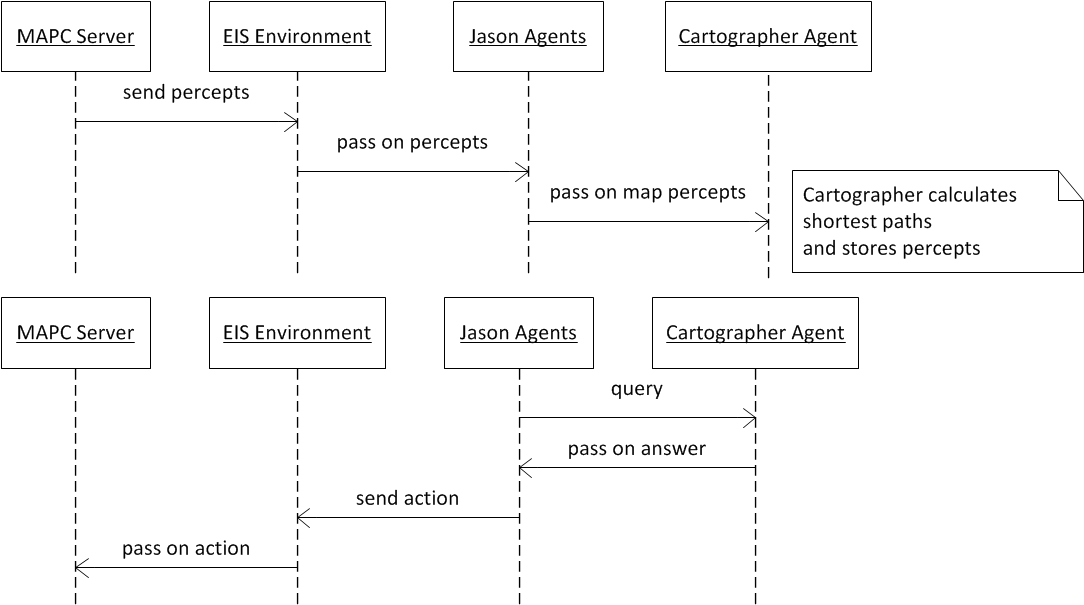
\includegraphics[width=\linewidth]{images/map_com_1.png}
  \caption{Initial communication approach for map generation.}
  \label{fig:map:com1}
\end{figure}

\begin{figure}
  \centering
  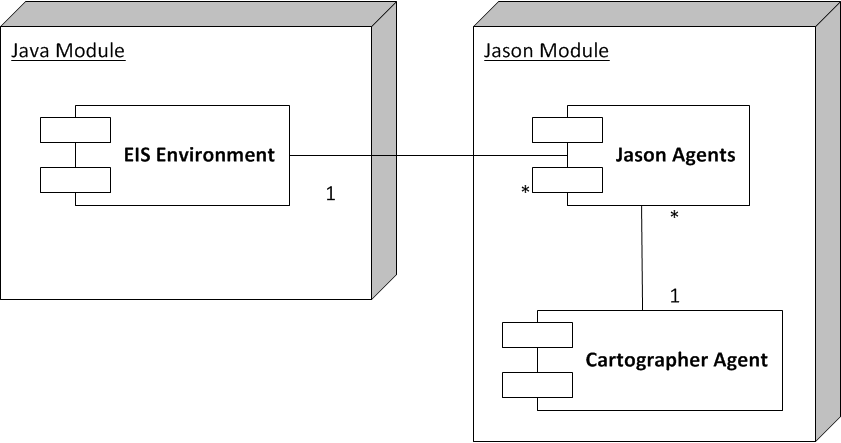
\includegraphics[width=\linewidth]{images/map_comp_1.png}
  \caption{Distribution of components between Jason and Java in our first approach.}
  \label{fig:map:comp1}
\end{figure}

Shortly after implementing this approach, we encountered two major problems, which both resulted in serious performance issues.
One problem came from our implementation of the pathfinding.
Although we used the Dijkstra-Algorithm, which is a efficient algorithm for this task, we encountered performance issues, because the pathfinding algorithm was executed every time an agent asked for a shortest path.
This led to a lot of redundant calculation and processing in the cartographer agent.
The second problem was related to communication between agents.
To understand the latter problem, one need to know that Jason uses a message box system for communication between agents.
This means that every message a sender sends to a receiver is queued in the receivers message inbox.
In every Jason lifecycle only one message is processed.
Although a Jason lifecycle is a lot shorter than a server lifecycle, after some execution time the inbox of the cartographer agent still was so full, that the processing of messages lagged far behind the receiving of these messages.
Both issues resulted in blocked agents, which had been waiting for the response of their queries for rounds.

To illustrate the problem assume the following example: A exploring agent comes to an unvisited vertex.
The first thing it does, is to ask the cartographer agent, whether this vertex was surveyed in the meantime.
After it gets the answer it surveys the vertex or asks the cartographer for the next unsurveyed vertex and travels there.
Then the whole procedure starts again.
As one can see, there are two possible bottlenecks.
The first one is the query for the state of an vertex and the second is the query for the next unsurveyed vertex, which includes calculating the shortest path to this vertex.
As described before the cartographer has not only to handle queries, but also handles map information input of every agent in every server cycle.
And due to the Jason communication approach this results in the cartographer not being able to handle queries immediate.
In our tests we saw answer times for queries around ten till twenty server cycles, which means that our agents were idle most of the time, waiting for answers from the cartographer agent.

%%%%%%%%%%%%%%%%%%
\subsubsection[Distance-Vector Routing Protocol]{Distance-Vector Routing-Protocol$^\star$}\label{alg:map_dv}
To solve the problem with repeating calculations of shortest paths we decided to calculate all shortest paths from the beginning and store these paths and other information in a network of ``node agents''.
\autoref{fig:map:com2} shows the second approach we used.
All percepts were passed through to the node agents.
Jason agents queried the respective node agent directly instead of querying the cartographer.
We extended our distribution model (see \autoref{fig:map:comp2}) to include the node agents.
\begin{figure}
  \centering
  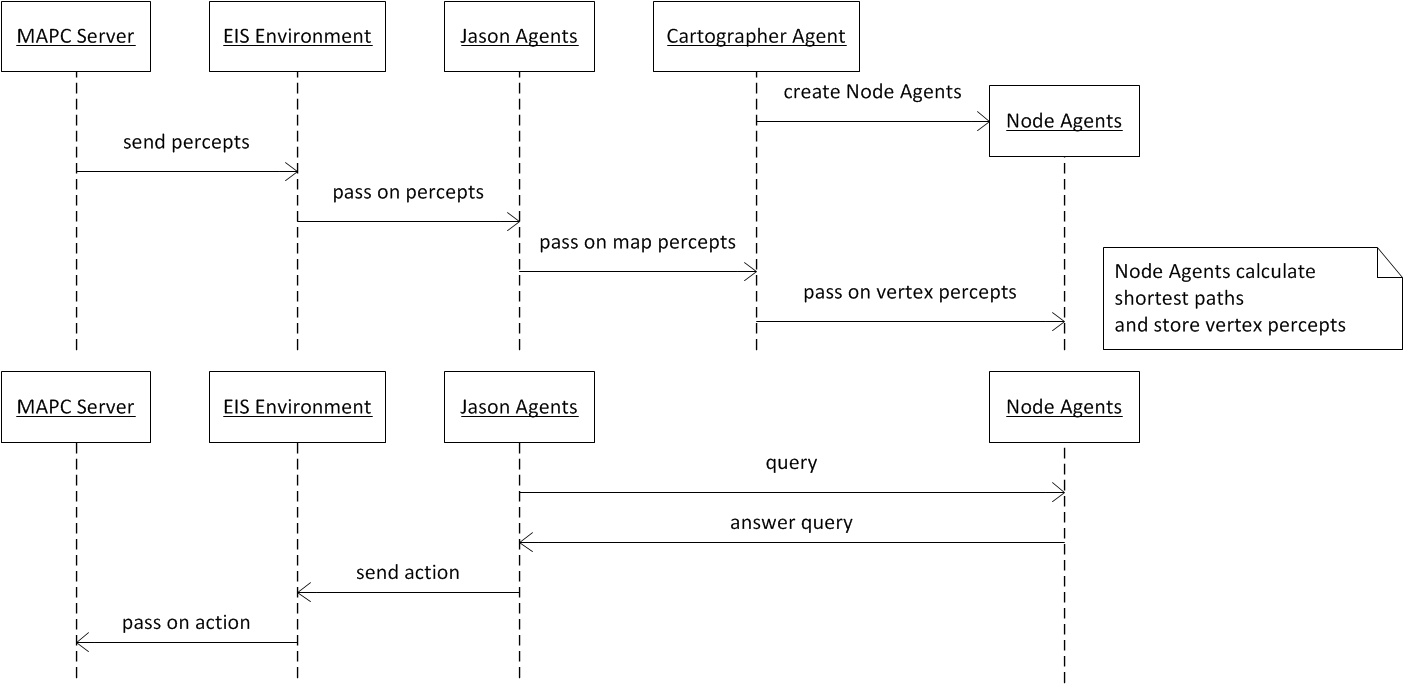
\includegraphics[width=\linewidth]{images/map_com_2.png}
  \caption{Second communication approach for map generation.}
  \label{fig:map:com2}
\end{figure}

\begin{figure}
  \centering
  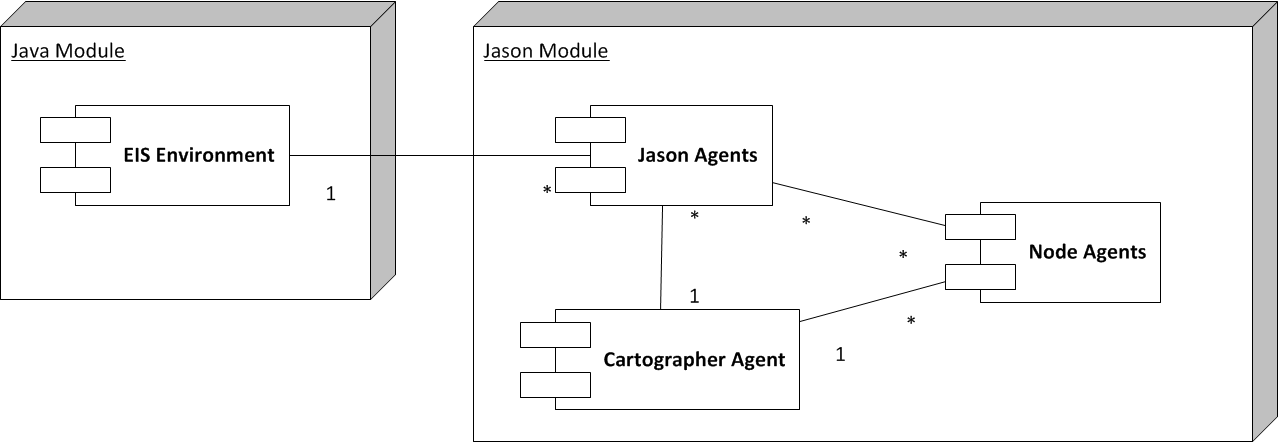
\includegraphics[width=\linewidth]{images/map_comp_2.png}
  \caption{Distribution of map components in our second approach.}
  \label{fig:map:comp2}
\end{figure}

A node agent represents one vertex of the scenario map and holds information about this vertex.
To make it easier to address node agents, we named node agents like the vertex they represented.
Node agent store all its neighbours in a neighbour-list belief (\texttt{neighbours([<ListOfNeighbours>])}) and all available paths to other vertices as path beliefs (\texttt{path(<Destination>, <NextHop>, <Hops>, <CostToNextHop>)}).
With regard to exploration and zoning we decided that an node agent also has to store the probed value of the vertex, and whether it was already probed or surveyed.
We changed the cartographer agents tasks, so that it only had to create the node agents at runtime.
All information input and queries now were directed to the respective node agents.

\begin{samepage}
The following list shows an example belief base of a node agent \texttt{v1}:
\begin{itemize}
  \item \texttt{neighbours([v2, v3]).}
  \item \texttt{probed(true).}
  \item \texttt{probedValue(7).}
  \item \texttt{surveyed(true).}
  \item \texttt{path(v1, v1, 0, 0).}
  \item \texttt{path(v2, v2, 1, 3).}
  \item \texttt{path(v10, v2, 4, 3).}
  \item \texttt{path(v8, v3, 3, 2).}
\end{itemize}
\end{samepage}

A query for a shortest path would look like this:
\begin{lstlisting}[caption={Query for shortest path from \texttt{v1} to \texttt{v8}}, label={lst:dv_shortestPath_query}]
  .send(v1, askOne, path(v8, NextHop, _, CostToNextHop)).
\end{lstlisting}
After looking up the belief in its belief base the node agent would unify the parameter \texttt{NextHop} with \texttt{v3} and CostToNextHop with \texttt{2} and response to the querying agent.

For propagating data between these node agents we used a modified \emph{Distance-Vector Routing Protocol} (short: DV).
DV is a routing protocol based on the Bellman-Ford algorithm and normally has its use in packet-switched networks.
DV can be executed on a network of nodes.
The basic idea is that each node informs all of its neighbour nodes about its belief base.
The informed nodes then update their belief base and also inform all of its neighbours and so on.
Because the Bellman-Ford algorithm has no loop detection, we had to implement some kind of break condition for the algorithm.
We used the value of the calculated shortest path as a termination condition.
If a new calculated path to another node agent is shorter than the already known path than the node agent has to inform its neighbours.
Otherwise it just does nothing.
At some point all information and paths are propagated through the whole network and all nodes have a consistent belief base.
\autoref{fig:dv} illustrates the algorithm for a small set of four neighbour nodes.

\begin{figure}
  \centering
  \caption{Executing the Distance-Vector Routing Protocol algorithm as described in \autoref{alg:map_dv} on a small network of four nodes. Each node has a table attached, containing all accessible nodes. The first parameter is the destination node, the second one is the node to pass through and the third parameter shows the overall distance to the destination.       \label{fig:dv}}
    \begin{subfigure}{.45\textwidth}
        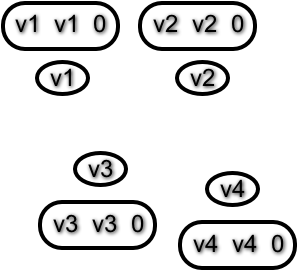
\includegraphics[width=\textwidth] {images/dv0.png}
        \caption{Initial set of node agents with their belief base. Each node agent knows only about itself and the shortest path to itself. The traveling costs to itself are zero.}
    \end{subfigure}\quad
    \begin{subfigure}{.45\textwidth}
        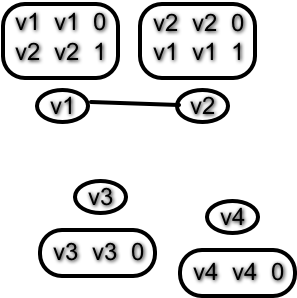
\includegraphics[width=\textwidth] {images/dv1.png}
        \caption{The node agents \texttt{v1} and \texttt{v2} are informed that they are neighbours. So they know that there must be a path to the other node agent. Because they are direct neighbours they are one hop away. \texttt{v3} and \texttt{v4} are not connected to the network right now, so they will not be informed about the path between \texttt{v1} and \texttt{v2}.}
    \end{subfigure}

    \begin{subfigure}{.45\textwidth}
       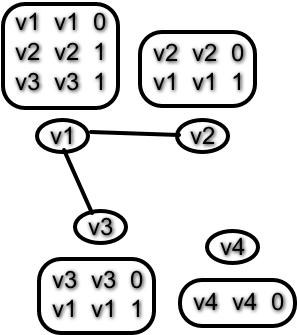
\includegraphics[width=\textwidth] {images/dv2.png}
       \caption{Now \texttt{v3} is added to the network by informing \texttt{v3} and \texttt{v1} about their neighbourhood relation. At first only \texttt{v1}  and \texttt{v3} update their belief base.}
    \end{subfigure}\quad
    \begin{subfigure}{.45\textwidth}
        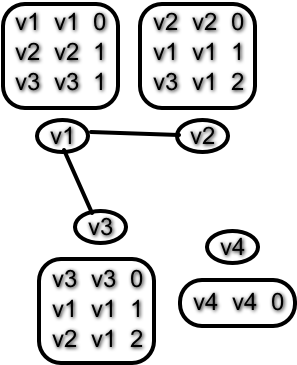
\includegraphics[width=\textwidth] {images/dv3.png}
        \caption{In the next step \texttt{v2} is informed about the path from \texttt{v1} to \texttt{v3}. \texttt{V2}  now knows that the shortest path to \texttt{v3} is by passing \texttt{v1} and that \texttt{v3} is 2 hops away.}
    \end{subfigure}
\end{figure}
\clearpage
\begin{figure}
  \centering
    \ContinuedFloat % continue from previous page
    \begin{subfigure}{.45\textwidth}
        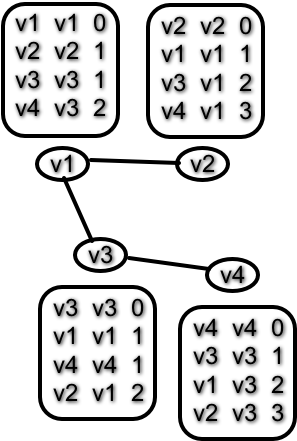
\includegraphics[width=\textwidth] {images/dv4.png}
       \caption{After that \texttt{v4} is added to the network and each node agent updates its belief base.}
    \end{subfigure}\quad
    \begin{subfigure}{.45\textwidth}
        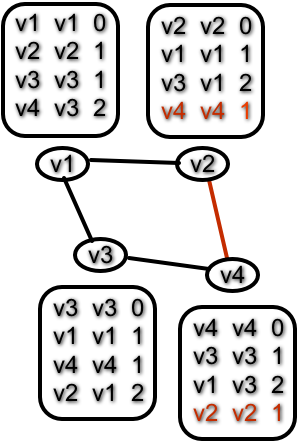
\includegraphics[width=\textwidth] {images/dv5.png}
        \caption{In the last step \texttt{v2} and \texttt{v4} are informed that they are neighbours. Because of that the shortest path between both node agents changes and is updated. The paths for the other node agents stay as is, because they can not get better. }
    \end{subfigure}
    \phantomcaption
\end{figure}

By distributing the information from one cartographer agent to a huge network of node agents we also distributed the load from one agent, the cartographer agent, on the respective node agents.
But we still had queries which were not answered immediate, because now we had a lot of communication going on between node agents.
Around 400 Jason agents were calculating shortest paths in parallel within the node agent networks and received at the same time information again and again by the exploring agents.
This information however was redundant in most cases, but still had to be processed.
This led to a high load on our system.
As a first step, we restricted communication between node agents and real agents.
The necessary map information was received directly from the Java EIS Environment module (short: JE).
The JE used a filter to ensure that only map information was sent to node agents that they were not aware of.
Since the message boxes now longer were flooded, communication between agents got a lot better.
But two reasons made us to discard this approach also and to change to a solution based entirely on Java.
First we were not able to reduce the load on our system by these changes.
Further we observed that some beliefs were not received by the node agents.
Even worse over the time beliefs disappeared from node agents belief bases.
Due to the constant high workload on our system, we saw that agents sent actions to the server too late, which led again to a lot of idle phases of our agents.

%%%%%%%%%%%%%%%%%%
\subsubsection[JavaMap]{JavaMap$^\star$}\label{alg:map_javamap}
We decided to implement the whole map module in Java.
This solved all of the previous described problems.
The JavaMap module gets its map information directly from the JE and is queried through internal actions by the Jason agents (see: \autoref{fun:apl_jason}).
Internally the JavaMap creates and manages a list of vertex-objects which are like the node agents from our previous approach.
Every vertex has stored a list of all paths it knows and alle vertex information.
This includes the one-hop neighbourhood and the probed value of the vertex.
\autoref{fig:map:com3} shows how the map percepts are now passed to the JavaMap and how Jason agents query the JavaMap.
\begin{figure}
  \centering
  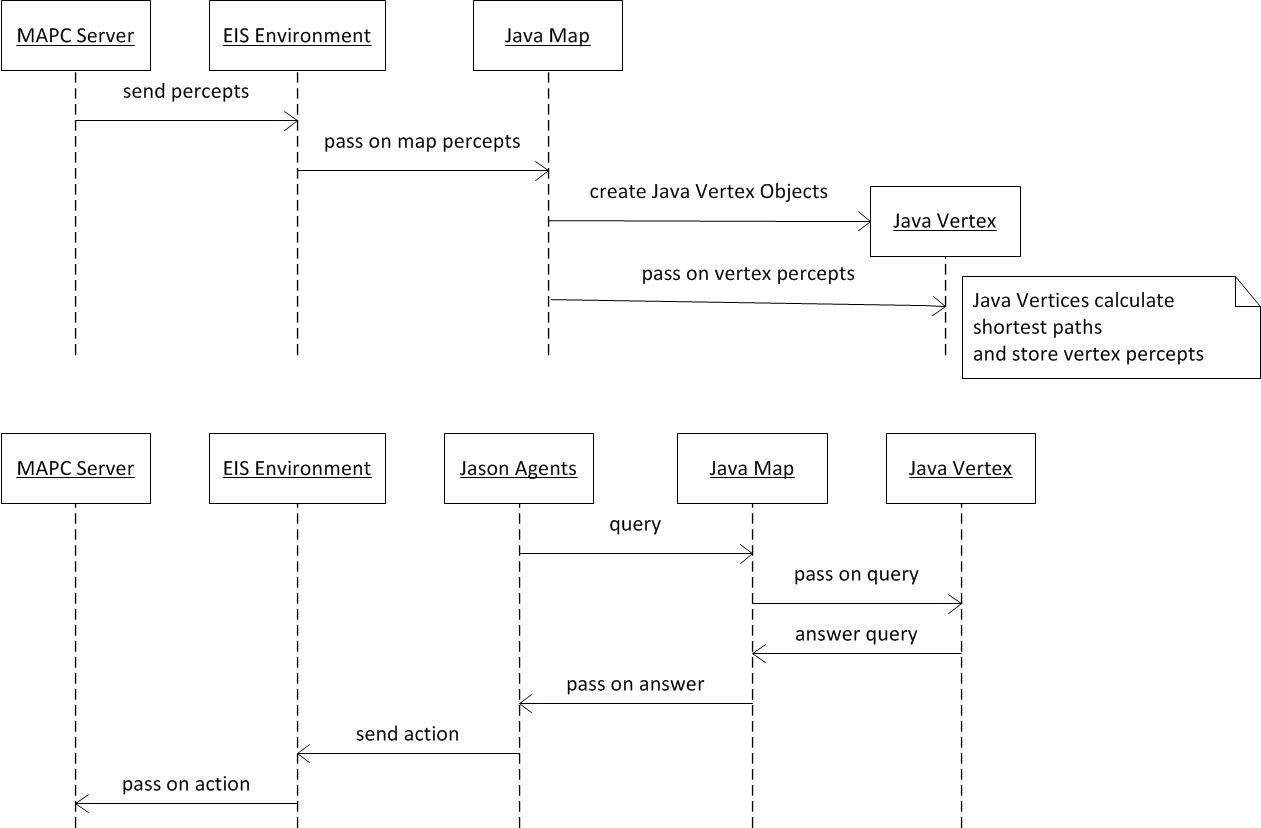
\includegraphics[width=\linewidth]{images/map_com_3.png}
  \caption{Final communication approach for map generation.}
  \label{fig:map:com3}
\end{figure}

In \autoref{fig:map:comp3} it is demonstrated how we changed the distribution of our components for map generation between Java and Jason. Unlike the first and second approach we now have a separation of concerns. The whole map generation and calculation is done entirely by Java and agent related actions and communication entirely in Jason.
\begin{figure}
  \centering
  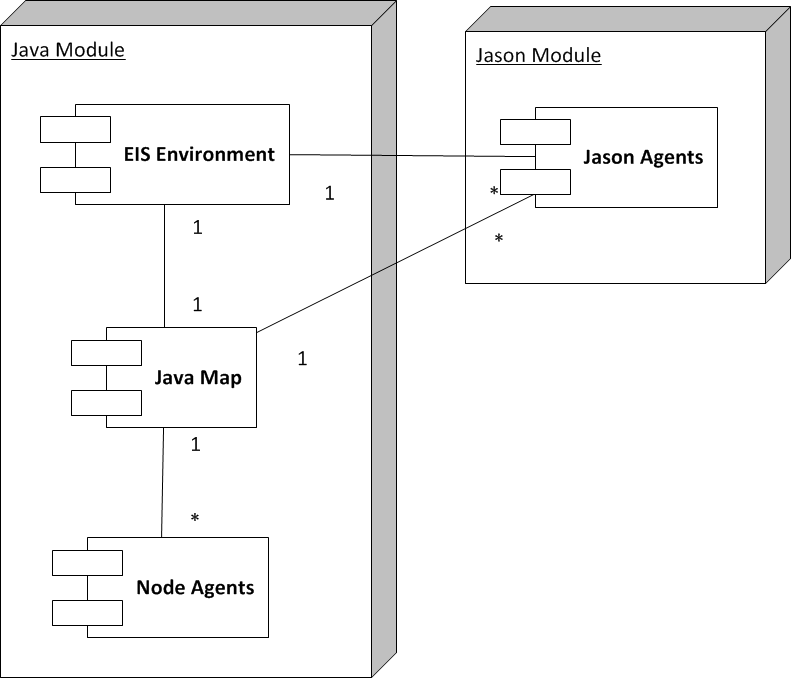
\includegraphics[width=\linewidth]{images/map_comp_3.png}
  \caption{Distribution of map components in our final solution.}
  \label{fig:map:comp3}
\end{figure}
